% !TEX TS-program = pdflatex
% !TEX encoding = UTF-8 Unicode

% This is a simple template for a LaTeX document using the "article" class.
% See "book", "report", "letter" for other types of document.

\documentclass[11pt]{article} % use larger type; default would be 10pt

\usepackage[utf8]{inputenc} % set input encoding (not needed with XeLaTeX)

%%% Examples of Article customizations
% These packages are optional, depending whether you want the features they provide.
% See the LaTeX Companion or other references for full information.

%%% PAGE DIMENSIONS
\usepackage{geometry} % to change the page dimensions
\geometry{a4paper} % or letterpaper (US) or a5paper or....
% \geometry{margin=2in} % for example, change the margins to 2 inches all round
% \geometry{landscape} % set up the page for landscape
%   read geometry.pdf for detailed page layout information

\usepackage{graphicx} % support the \includegraphics command and options

% \usepackage[parfill]{parskip} % Activate to begin paragraphs with an empty line rather than an indent

%%% PACKAGES
\usepackage[spanish]{babel}
\usepackage{booktabs} % for much better looking tables
\usepackage{array} % for better arrays (eg matrices) in maths
\usepackage{paralist} % very flexible & customisable lists (eg. enumerate/itemize, etc.)
\usepackage{verbatim} % adds environment for commenting out blocks of text & for better verbatim
\usepackage{subfig} % make it possible to include more than one captioned figure/table in a single float
% These packages are all incorporated in the memoir class to one degree or another...

%%% HEADERS & FOOTERS
\usepackage{fancyhdr} % This should be set AFTER setting up the page geometry
\pagestyle{fancy} % options: empty , plain , fancy
\renewcommand{\headrulewidth}{0pt} % customise the layout...
\lhead{}\chead{}\rhead{}
\lfoot{}\cfoot{\thepage}\rfoot{}

%%% SECTION TITLE APPEARANCE
\usepackage{sectsty}
\allsectionsfont{\sffamily\mdseries\upshape} % (See the fntguide.pdf for font help)
% (This matches ConTeXt defaults)

%%% ToC (table of contents) APPEARANCE
\usepackage[nottoc,notlof,notlot]{tocbibind} % Put the bibliography in the ToC
\usepackage[titles,subfigure]{tocloft} % Alter the style of the Table of Contents
\renewcommand{\cftsecfont}{\rmfamily\mdseries\upshape}
\renewcommand{\cftsecpagefont}{\rmfamily\mdseries\upshape} % No bold!

%%% END Article customizations

%%% The "real" document content comes below...

\title{Procesamiento de archivos  XML  en Haskell}
\author{Lozano E. , Alvarado J \& .Lasso H}
%\date{} % Activate to display a given date or no date (if empty),
         % otherwise the current date is printed 

\begin{document}
\maketitle

\section{Introducción}
El propósito de nuestro proyecto es realizar un parseo de XML a una estructura manejable en Haskell. Este parseo se realiza para poder consultar y manipular datos totales, o ciertas especificaciones en una lista de 15438 Dispositivos con sus respectivas características. Esta lista es creada en base a la lectura de un archivo XML y a datos de tipos definidos por nosotros en Haskell, como lo son: Device, Group y Capability. \\
\\ Haskell es un lenguaje de programación puramente funcional, éste permite decirle al computador no como tiene que hacer las tareas, sino más bien como están definidas. Es elegante y conciso ya que utiliza conceptos de alto nivel. Los programas Haskell son normalmente más cortos que los equivalentes imperativos por tanto es más eficiente su mantenimiento y además poseen menos errores.

\section{Alcance}
El alcance de nuestro proyecto Haskell es realizar la lectura de un archivo XML, manipular y analizar su contenido y representarlo en una estructura de tipo Lista en Haskell para realizar funciones de consulta o de busqueda.

\section{Descripción}

XML se puede considerar como un lenguaje que en sus documentos usa una estructura recursiva. Y eso a nuestro favor permite que Haskell manipule los módulos enteros del archivo con su mejor característica: Recursividad.\\ \\
La recursividad en nuestro proyecto Haskell la usamos para poder manipular el archivo XML y reconocer que tipo de dato es el que encontramos en cada etiqueta de apertura y de cierre. Es decir las definidas con los simbolos de mayor o menor: $<$f$>$abc$<$/f$>$. Estas etiquetas pueden ser en parejas  ( $<$f$>$ ,$<$/f$>$) o únicas (apertura y cierre) ($<$f ... /$>$). Y que recursivamente pueden contener más parejas de etiquetas o texto plano.\\ \\ \\
Haskell incluye el soporte para los tipos de datos y funciones recursivas, Listas, Guardas y Tuplas. Por tanto el uso de este lenguaje es práctico a la hora de leer y representar un documento XML. Que es lo que buscamos. \\  De hecho, las combinaciones de estas características de Haskell pueden resultar en algunas funciones muy sencillas cuya versión usando lenguajes imperativos, puede llegar a resultar extremadamente tediosa de programar.
\\ \\
Gracias a esta funcionalidad de Haskell nuestra decisión de programación fue leer el documento XML y su conjunto de datos, para representarlo como una Lista. Pero no una Lista de Enteros o de Cadenas de Texto sino una Lista de un Tipo de Dato. \\ Haskell permite que definamos un Dato con sus características y a su vez el Tipo de Dato de las mismas. Por lo que definimos tres de estas en nuestro proyecto: Device, Group y Capability. Y al final lo que tuvimos como resultado fue una Lista que almacena Device.
\begin{center}
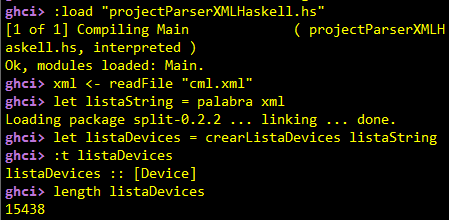
\includegraphics[scale=0.7]{Imagenes/CargarDevices.png}
\end{center}
Un Device tiene como características:  idD de Tipo String, user\_agent de Tipo String, fall\_back de Tipo String y una Lista que almacena los grupos que contiene el Device de Tipo [Group].\\
Un Group tiene como características: idG de Tipo String y una Lista que almacena las capabilities que pertenecen a ese Group que son de Tipo [Capability].\\
Una Capability tiene como características: name de Tipo String y value de Tipo String.\\ \\
Es de notar que es una forma muy eficiente de interpretar el XML, ya que como resultado obtenemos una Lista de Device que es más útil a la hora de manipular que el XML cómo tal. Por ejemplo un Device corto de la lista sería el siguiente:
\begin{center}
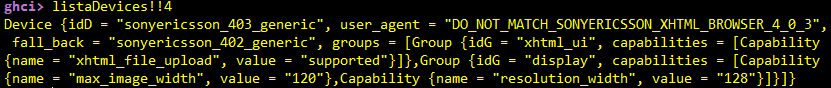
\includegraphics[scale=0.7]{Imagenes/EjempDevice.png}
\end{center}
\section{¿Qué se implementó y qué no se implementó? }
\subsection{Lo implementado} 
Una vez leido y manipulado el contenido del archivo xml, la representamos en una lista de Devices que contiene elementos de tipo Device , cada Device contiene una lista de Groups que tienen elementos de tipo Group y cada Group contiene una lista  de  Capabilities que tienen elementos de tipo Capability.  
Con la lista de Devices  ya obtenida podemos consultar la información de cada Device, Group o Capability. Un ejemplo sería el siguiente:
\begin{center}
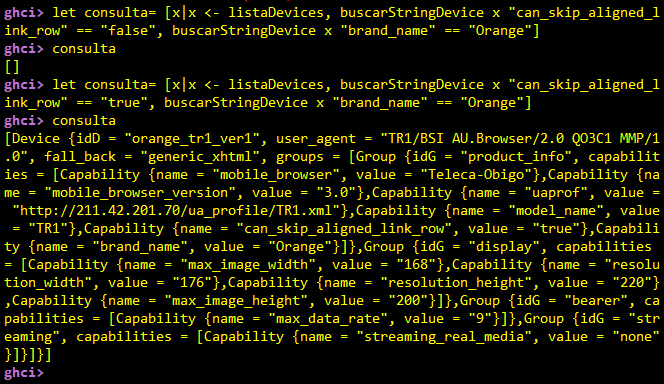
\includegraphics[scale=0.7]{Imagenes/Consulta.png}
\end{center}
En estos dos ejemplos vemos a la función de busqueda retornando una lista vacia como una lista con un solo dispositivo que cumpla las características que buscamos. La función ``buscarStringDevice” es para poder encontrar todos los Devices que tengan esas Capabilities.
\subsection{Lo no implementado} 
Todos los requerimientos del proyecto han sido implementados.

\section{Observaciones}
\begin{itemize}
\item Aprender a programar en Haskell no fue sencillo, ya que para aquellos que estamos acostumbrados a lenguajes de programación imperativos es bastante abstracto aplicar en todas las funciones recursividad. Nos quedó claro que Haskell no posee estructuras de control y de flujo, y el porqué. Fue interesante leer e investigar sobre Haskell ya que salimos de la rutina de programación para entender que las estructuras de repetición (for, while...) no siempre son mejores que la recursividad.

\end{itemize}
\section{ Conclusiones}

\begin{itemize}
\item Conocer y trabajar con nuevos lenguajes nos ayuda a comprender que distintas tareas se pueden resolver de distintas maneras y con diferentes criterios. Pero que siempre el fin es buscar simplificar la solución y sin complicaciones que muchas veces son evitables.
\item Representar la información del archivo XML que nos proporciona información de distintos Dispositivos en una estructura sencilla, nos ayuda hacer consultas de una manera mas eficiente. 
\item La recursividad en muchos casos ahorra lineas de código que las estructuras de repetición, por lo que facilita el mantenimiento del código y a su vez permite disminuie la cantidad de errores. 
\end {itemize}

\end{document}
